\documentclass[nofootinbib,amssymb,amsmath]{revtex4}
\usepackage{mathtools}
\usepackage{amsthm}
\usepackage{algorithm}
\usepackage{algpseudocode}
\usepackage{lmodern}
\usepackage{graphicx}
\usepackage{color}
\usepackage{mathrsfs}

%Put an averaged random variable between brackets
\newcommand{\ave}[1]{\left\langle #1 \right\rangle}

\newcommand{\vzero}{{\bf 0}}
\newcommand{\vI}{{\bf I}}
\newcommand{\vb}{{\bf b}}
\newcommand{\vd}{{\bf d}}
\newcommand{\vc}{{\bf c}}
\newcommand{\vv}{{\bf v}}
\newcommand{\vz}{{\bf z}}
\newcommand{\vn}{{\bf n}}
\newcommand{\vm}{{\bf m}}
\newcommand{\vG}{{\bf G}}
\newcommand{\vQ}{{\bf Q}}
\newcommand{\vM}{{\bf M}}
\newcommand{\vW}{{\bf W}}
\newcommand{\vX}{{\bf X}}
\newcommand{\vF}{{\bf F}}
\newcommand{\vZ}{{\bf Z}}

\newcommand{\vPsi}{{\bf \Psi}}
\newcommand{\vSigma}{{\bf \Sigma}}
\newcommand{\vlambda}{{\bf \lambda}}
\newcommand{\vLambda}{{\bf \Lambda}}
\newcommand{\vtheta}{{\boldsymbol \theta}}
\newcommand{\vpi}{{\boldsymbol \pi}}
\newcommand{\vA}{{\bf A}}
\newcommand{\MM}{M}
\newcommand{\PP}{\mathcal{P}}
\newcommand{\EE}{\mathbb{E}}
\newcommand{\norm}{{\mathcal N}}

\newtheorem{lemma}{Lemma}
\newtheorem{corollary}{Corollary}

\def\SL#1{{\color [rgb]{0,0,0.8} [SL: #1]}}
\def\DB#1{{\color [rgb]{0,0.8,0} [DB: #1]}}

\newcommand{\epss}{\varepsilon}

\DeclarePairedDelimiter\ceil{\lceil}{\rceil}
\DeclarePairedDelimiter\floor{\lfloor}{\rfloor}

\makeatletter
\DeclareFontFamily{OMX}{MnSymbolE}{}
\DeclareSymbolFont{MnLargeSymbols}{OMX}{MnSymbolE}{m}{n}
\SetSymbolFont{MnLargeSymbols}{bold}{OMX}{MnSymbolE}{b}{n}
\DeclareFontShape{OMX}{MnSymbolE}{m}{n}{
    <-6>  MnSymbolE5
   <6-7>  MnSymbolE6
   <7-8>  MnSymbolE7
   <8-9>  MnSymbolE8
   <9-10> MnSymbolE9
  <10-12> MnSymbolE10
  <12->   MnSymbolE12
}{}
\DeclareFontShape{OMX}{MnSymbolE}{b}{n}{
    <-6>  MnSymbolE-Bold5
   <6-7>  MnSymbolE-Bold6
   <7-8>  MnSymbolE-Bold7
   <8-9>  MnSymbolE-Bold8
   <9-10> MnSymbolE-Bold9
  <10-12> MnSymbolE-Bold10
  <12->   MnSymbolE-Bold12
}{}

\let\llangle\@undefined
\let\rrangle\@undefined
\DeclareMathDelimiter{\llangle}{\mathopen}%
                     {MnLargeSymbols}{'164}{MnLargeSymbols}{'164}
\DeclareMathDelimiter{\rrangle}{\mathclose}%
                     {MnLargeSymbols}{'171}{MnLargeSymbols}{'171}
\makeatother

\begin{document}

\title{A probabilistic model for coverage bias estimation and CNV detection}

\author{Mehrtash Babadi}
\email{mehrtash@broadinstitute.org}
\affiliation{Broad Institute, 75 Ames Street, Cambridge, MA 02142}

\author{David Benjamin}
\email{davidben@broadinstitute.org}
\affiliation{Broad Institute, 75 Ames Street, Cambridge, MA 02142}

\author{Samuel K. Lee}
\email{slee@broadinstitute.org}
\affiliation{Broad Institute, 75 Ames Street, Cambridge, MA 02142}

\date{\today}

\begin{abstract}
These notes exclusively cover the target coverage model in the GATK CNV pipeline.
\end{abstract}

\maketitle

\section{Introduction}
\noindent We wish to address several goals in this section:

\begin{itemize}

\item Connect copy ratio (or copy number) and raw read counts in a single sensible probabilistic model without heuristic data transformation.

\item Take into account the Poisson nature of coverage depth, thereby giving less weight to low-coverage targets and separating the inherent variance due to Poisson statistics from experimental noise. We want to use the panel of normals to subtract only the latter.

\item Choose the number of principal components to use in an automatic and principled manner.

\item Use an algorithm that does not waste time calculating all principal components when we only want the few most significant ones.

\item Make a universal panel of normals for both sexes by taking into account both autosomal and allosomal targets. This requires the flexibility to handle samples with ``missing data''.

\item Correct for CNV events that occur in the panel of normals.

\item Regularize the model property to ensure biological CNV events and laboratory biases are separable from each other, in particular when dealing with a small number of samples.

\end{itemize}

\subsection{Notation}
We use bold symbols for vectors and matrices (e.g. $\mathbf{n}$) and the corresponding regular symbols when the indices are explicitly written (e.g. $n_{st}$). We use the notation $\mathbf{n}_s$ to refer to the $s$ row vector of the full matrix $\mathbf{n}$. Roman indices are used for sample and target indices whereas Greek indices are reserved for latent space indices.

\section{The model}
Suppose we have vectors of read counts over a set of $T$ targets for $S$ samples, $\vn_s, \, s = 1 \ldots S$ where $n_{st}$ is the coverage of sample $s$ at target $t$. In order to include both sexes on an equal footing, we further define a ``germline ploidy matrix'' $\PP_{st}$ such that $\PP_{st}$ is the germline ploidy\footnote{For human autosomal targets, $\PP_{st} = 2$ for both sexes. In female samples, $P_{st} = 2$ for X chromosome targets and $P_{st} = 0$ for Y chromosome targets. Finally, $P_{st} = 1$ for X and Y chromosomes in male samples} of target $t$ of sample $s$. We imagine that laboratory conditions for a particular sample yielding an underlying bias vector $\vb_s$, where $e^{b_{st}}$ is the propensity of target $t$ to be captured, sequenced, and mapped in the preparation of sample $s$. Suppose also that sample $s$ has an average depth $d_s$ and a vector of copy numbers $\vc_s$, where the latent variable $c_{st}$ is the copy number of sample $s$ at target $t$. Our model for read counts is:
%
\begin{equation}
n_{st} \sim {\rm Poisson}(d_s \PP_{st} c_{st} e^{b_{st}})
\label{coverage_model}
\end{equation}
We can achieve many of the goals listed above by performing probabilistic principal component analysis (PCA) not on directly $\vn$, but rather on $\vb$. One one hand, the Poisson parameters must be positive and therefore, $\exp(\vb)$ is a well-defined parametrization of the multiplicative bias. On the other hand, a Gaussian model for $\vb$ implies a log-normal distribution for $\exp(\vb)$ which is indeed the expected distribution when the multiplicative bias arises from several independent sources according to the central limit theorem\footnote{Let $B = \prod_{j=1}^{N_B} B_j$ be the total multiplicative bias where $B_j \in (0, \infty)$ are independent components of the bias. For $N_B \gg 1$, $\ln(B) \sim \mathcal{N}$ and therefore, $B$ has a log-normal distribution.}. We model $\vb_s$ as:
%
\begin{align}
\vz_s &\sim \norm(\vzero, \vI), \nonumber\\
\vb_s &\sim \norm(\vW \vz_s + \vm, \vPsi),
\end{align}
%
where $\vz_s \in \mathbb{R}^D$ is a low-dimensional latent vector representing laboratory conditions, $\vW \in \mathbb{R}^{T \times D}$ is a linear map from latent space to target space, $\vm \in \mathbb{R}^T$ is the vector of mean biases, and $\vPsi \in \mathbb{R}^{T \times T}$ is a diagonal matrix of residual variance not explained by the latent features. We approximate the Poisson as a Gaussian and expand the argument of the Gaussian exponential about the mode of $b_{st}$ to quadratic order to obtain:
%
\begin{equation}\label{eq:gaussian_approx_coverage}
{\rm Poisson}(n_{st} | d_s \PP_{st} c_{st} e^{b_{st}}) \simeq \Sigma_{st} \, \norm(b_{st} | m_{st}, \Sigma_{st}),
\end{equation}
where:
\begin{align}
m_{st} &\equiv \ln(n_{st}/\PP_{st}) - \ln (c_{st}) - \ln(d_s), \nonumber\\
\Sigma_{st} &\equiv 1/n_{st}.
\label{eq:m_sigma_def}
\end{align}

\begin{figure}
\center
\includegraphics[scale=0.7]{figs/{gauss_poisson_0.1}.pdf}
\includegraphics[scale=0.7]{figs/{gauss_poisson_10}.pdf}
\caption{Gaussian approximation to the Poisson likelihood (see Eq.~\ref{eq:gaussian_approx_coverage}). The left and right panels show $\mathrm{Poisson}(n|\alpha\,e^b)$ and $n^{-1}\mathcal{N}(b|\ln(n/\alpha), n^{-1})$, respectively for $\alpha=0.1$ (top) and $\alpha=10.0$ (bottom). The black lines show $b = \ln(n/\alpha)$ the maximum likelihood bias estimate. The Gaussian approximation breaks down at $n=0$ (no coverage). It also slightly overestimates the variance at small $n$. Otherwise, it is an excellent approximation.}
\label{fig:gaussian_approx_coverage}
\end{figure}

Note that $\Sigma_{st}$ can be thought of as the width of the distribution of $b_{st}$ about its maximum likelihood estimate such that in the limit $n_{st}, d_s \rightarrow \infty$, ${\rm Poisson}(n_{st} | d_s c_{st} e^{b_{st}}) \rightarrow \delta(b_{st} - b^*_{st})$ where $b^*_{st} = \lim_{n,d \rightarrow \infty} m_{st}$ is the true bias. The above approximation, while being excellent for well-covered targets (see Fig.~\ref{fig:gaussian_approx_coverage}), inevitably breaks down for targets that are uncovered {\em ex ante} in some samples, such as $Y$ chromosome targets in female samples. To this end, we define a ``sample-target mask matrix'' $\MM_{st}$ such that $\MM_{st} = 0$ if $\PP_{st} = 0$, and $\MM_{st} = 1$ if $\PP_{st} \neq 0$, and for each sample-target pair $(s,t)$, we only consider targets where the $\MM_{st} \neq 0$ in the joint likelihood function. The latter is thus written as:
\begin{equation}
P(n_{st}, b_{st}, z_{st}, d_s | c_{st}, \vtheta) \propto \norm(\vz_s | \vzero, \vI) \, \Big[\norm(b_{st} | (\vW \vz_s)_t + m_t, \Psi_t) \, \norm(b_{st} | m_{st}, \Sigma_{st})\Big]^{M_{st}},
\end{equation}
where $\vtheta = (\vW, \vm, \vPsi)$ denote the parameters we wish to learn. We can integrate out $b_{st}$ readily to obtain\footnote{The integration is easily performed using the identity $\int_{-\infty}^{+\infty} \norm(x | \mu_1, \sigma_1^2) \, \norm(x | \mu_2, \sigma_2^2) \, \mathrm{d}x = \norm(\mu_1 | \mu_2, \sigma_1^2 + \sigma_2^2)$.}:
%
\begin{equation}
P(n_{st}, z_{st}, d_s | c_{st}, \vtheta) \propto \norm(\vz_s | \vzero, \vI) \, \Big[\norm(m_{st} | (\vW \vz_s)_t + m_t, \Psi_{st})\Big]^{M_{st}},
\label{coverage_likelihood}
\end{equation}
where we have defined:
\begin{equation}
\Psi_{st} = \Psi_t + \Sigma_{st}.
\label{eq:psi_def}
\end{equation}
We model the copy number states (or copy ratios in case of somatic samples) using a finite state hidden Markov model (HMM). Put together, we obtain:
\begin{equation}
P(\vn_s, \vz_s, \vc_s, d_s | \vtheta) \propto \left[P(c_{s,0}|\vpi) \prod_{t=1}^{T-1}P(c_{s,t}| c_{s,t-1}, \mathbf{T}_t)\right] \left[\prod_{t=0}^{T-1} P(n_{st}, z_{st} | c_{st}, \vtheta)\right].
\label{eq:complete_log_likelihood}
\end{equation}
Here, $\vpi$ is a vector denoting the prior probabilities of various copy number states, and $\mathbf{T}_t$ is the transition matrix at target $t$. We treat HMM parameters as given (hyperparameters).\\

It is illuminating to study Eq.~\eqref{coverage_likelihood} before we proceed. To this end, we marginalize the bias latent variable $\vz_s$ in Eq.~\eqref{coverage_likelihood} to obtain the incomplete-data likelihood function. The final result can be put in a simple form using the Woodbury identity and properties of projection matrices:
%
\begin{equation}
P(\vn | \vc, \vtheta) \propto \exp \left( -\frac{1}{2} \sum_s (\vm_s - \vm)^T \vM_s (\vPsi + \vSigma_s + \vM_s \vW \vW^T \vM_s)^{-1} \vM_s (\vm_s - \vm) \right),
\label{marginalized coverage_likelihood}
\end{equation}
%
where $\vM_s$ and $\Sigma_{s}$ are $T \times T$ diagonal matrices having $M_{st}$ and $\Sigma_{st}$ in their diagonal entries, respectively. The incomplete-data likelihood function poses a Gaussian distribution for $\ln(n_{st})$ (See Eq.~\ref{eq:m_sigma_def}). The covariance matrix is the diagonal in the target space and is composed of three terms: (1) $\vPsi$ target-specific ``unexplained'' noises, (2) $\vM_s \vW \vW^T \vM_s$ denotes the ``explained'' variance due to laboratory conditions, and (3) $\Sigma_{st} = 1/n_{st}$ denotes the statistical variance in read counts, it has roots in the Poisson distribution for read counts, and can be thought of as a penalty factor that decreases the role of lower-coverage samples in the likelihood.

\subsection{A Laplace regularization scheme for separating latent features from biological CNV events}
PCA-like approaches to denoising aim at minimizing the {\em total variance} of the data by learning and subtracting the contribution of the underlying latent features. In practice, this objective is achieved using either the maximum variance principle (usual PCA) or the maximum likelihood principle on a linear-Gaussian model as explained here. Using either method, when the number of samples largely exceeds the dimension of the latent space, sample-specific variations become immaterial and the true underlying latent features can be learned from the data. However, when the number of samples is comparable to the number of latent features, the statistical power for separating sample-specific variations from mutual variations is significantly reduced.

Let us assume that we have an oracle for the first few major latent features, and that we have already subtracted the contribution arising from these features. Let $\sigma_\ell^2$ be the variance associated with the next leading latent feature. Subtracting this latent feature reduces the total variance by $S\sigma_\ell^2$, where $S$ is the number of samples. Now, if one of the samples has an individual leftover variance of magnitude $\sigma_s^2$ such that $\sigma_s^2 \gtrsim S\sigma_\ell^2$, then the maximum variance principle implies choosing the next principal component along the direction of that specific sample. In other words, the procedure erroneously learns a sample-specific signal as a source of noise. Note that this artifact occurs only if $S \lesssim \sigma_s^2 / \sigma_\ell^2$.\\

\noindent {\bf What is at stake? ---} There is no obvious theoretical guarantee for the MLE problem for $\vtheta$ to be convex. In all likelihood, if one of the samples has a large germline CNV event, it may be picked up as a principal component and be interpreted as experimental noise such that the MAP estimator for $\vc$ fails to call that CNV event. It is possible that the likelihood function has numerous such local maxima. Therefore, we wish to ensure that sample-specific {\em nuisances} are not picked up as Gaussian noise, no matter how strong they are. We discuss a number of such approaches in what follows.\\

\noindent {\bf (Idea 1) Blind source separation ---} One remedy is to use a blind source separation approach, such as independent component analysis (ICA), to separate the signal from the noise as a first step, followed by learning the latent features of the noise using PCA. In ICA-like methods, one decomposes the signal into additive subcomponents and minimizes the mutual information between them (or maximizes the non-Gaussianity by taking into account higher moments such as the kurtosis). Even though this method is quite appealing, we follow a more context-specific heuristic approach here.\\

\noindent {\bf (Idea 2) Employing a CNV-sensitive regularizer ---} Fortunately, we have some idea about the spatial structure of the CNV events: they are amplification or attenuation of the read count over several consecutive targets. In the absence of noise, we expect the frequency spectrum of the CNV signal (as obtained by taking a Fourier transform of $m_{st}$ in $t$) to be significantly enhanced at spatial frequencies corresponding to the inverse length scale of the size of the CNV event. Similarly, the variation subtracted from sample $s$, i.e. $\vW \vz_s$, will exhibit an enhanced spectral power if a CNV event is erroneously picked up. Let $\tilde{f}(k)$ be the Fourier transform of a linear filter that approximately represents a range of CNV events. For example, we may use a midpass filter such as:
\begin{equation}
\tilde{f}(k) = \left\{
\begin{array}{ll}
  1 & \quad k_l \leq k^* \leq k_h,\\
  \\
  0 & \quad k^* > k_h \,\, \text{or} \,\, k^* < k_l,
\end{array}
\right.
\end{equation}
Here, $k^* = \min(k, T - 1 - k)$, $k_l \sim \lfloor T / \ell_\mathrm{max} \rfloor$ and $k_l \sim \lfloor T / \ell_\mathrm{min} \rfloor$, where $\ell_\mathrm{min}$ and $\ell_\mathrm{max}$ denote roughly the minimum and maximum length of the CNV events in the units of targets. The filtered spectral power of the noise in sample $s$ is given as:
\begin{equation}
\kappa_s \equiv \sum_{k=0}^{T-1} \tilde{f}(k) \left|\mathrm{FFT}\left[\vW \vz_s\right]_k\right|^2 = \frac{1}{T}\sum_{t,t'=0}^{T-1}F_{tt'} \, W_{t\mu} \, W_{t'\nu} \, z_{s\mu} \, z_{s\nu},
\end{equation}
where $F_{tt'} = f(t-t') \equiv T^{-1} \sum_{k=0}^{T-1} e^{2\pi i k (t-t')/T} \tilde{f}(k)$ is the inverse DFT of $\tilde{f}(k)$. Now, in order to avoid picking up event-like variations as noise, we simply penalize variations with large $\kappa$. To this end, we regularize the coverage likelihood function Eq.~\eqref{coverage_likelihood} with the following Laplace penalty:
\begin{equation}
R_f \equiv \exp\left(-\frac{\lambda}{2} \sum_{s=1}^S\kappa_s\right) = \exp\left(-\frac{\lambda}{T}\sum_{s=1}^S\sum_{t,t'=1}^{T-1}f(t-t') \, W_{t\mu} \, W_{t'\nu} \, z_{s\mu} \, z_{s\nu}\right).
\end{equation}
We will discuss a proper choice of $\lambda$ later. 

\subsection{Automatic relevance determination (ARD) prior on $\vW$}
The true dimension of the latent space is not known a priori. When abundant data is available (i.e. $S \gg D_\mathrm{true}$), this problem can be addressed using the automatic relevance determination (ARD) technique. To this end, one starts with a liberal estimate for $D$ and imposes a Gaussian prior on $\vW$:
\begin{equation}
P(\vW) \propto \prod_\mu \alpha_\mu^{T/2} \exp \left( -\frac{1}{2} \alpha_\mu \sum_t W_{t\mu}^2  \right).
\label{eq:ARD_prior}
\end{equation}
If $\alpha_\mu \rightarrow \infty$, the latent feature $\mu$ is effectively turned off whereas if $\alpha_\mu \rightarrow 0$, the flat prior is recovered. The recipe for ARD is to initially set $\alpha_\mu \simeq 0$ while calculating and maximizing the model evidence $P(\vn | \{\alpha_\mu\}$ with respect to $\{\alpha_\mu\}$. If $D > D_\mathrm{true}$, we expect $D - D_\mathrm{true}$ elements of $\{\alpha_\mu\}$ to run to infinity. If $D_\mathrm{true}$, all of $\{\alpha_\mu\}$ will remain of the same order, signaling the necessity of increasing $D$.

\section{Mean-field variational EM algorithm}
Let us start by writing out the complete-data log likelihood (see Eq.~\ref{eq:complete_log_likelihood}), including the ARD prior and the Laplace regularizer:
\begin{subequations}
\begin{align}
\label{eq:complete_log_likelihood}
\ln P(\vn, \vc, \vz, \vd | \vtheta) &= \sum_{s} \ln P_\mathrm{HMM}\big(\vc_s \big|\vpi, \{\mathbf{T}_t\}\big) - \frac{1}{2}\sum_{st} M_{st} \, \bigg\{\ln \Psi_{st} + \Psi_{st}^{-1}\Big[(\vW \vz_s)_t^2 + \Delta_{st}^2 - 2\Delta_{st} (\vW \vz_s)_t\Big]\bigg\}\nonumber\\
& - \frac{\lambda}{2}\left(\frac{1}{T}\sum_{s=1}^S\sum_{t,t'=0}^{T-1}f(t-t') \, W_{t\mu} \, W_{t'\nu} \, z_{s\mu} \, z_{s\nu}\right) - \sum_{\mu=1}^{D}\left(\frac{T}{2} \, \ln \alpha_\mu -\frac{\alpha_\mu}{2} \sum_{t=0}^{T-1} W_{t\mu}^2  \right) + \mathrm{const.},\\
\label{eq:delta_def}
\Delta_{st} &= \ln(n_{st}/\PP_{st}) - \ln c_{st} - \ln d_s - m_t.
\end{align}
\end{subequations}
We notice that the latent variables $(\vc, \vd)$ are coupled to $\vz$ due to the cross term $\Delta \vW \vz$, resulting in an intractable E step. Intuitively, we expect the posterior distribution of $\vz$ to be quite narrow near the optimal solution provided $D_\mathrm{true} \ll T$. Therefore, we do not foresee the coupling to play a substantial role. This motivates the introduction of a factorized variational ansatz for the latent posterior distribution:
\begin{equation}
P(\vc, \vz, \vd | \vn, \vtheta) \simeq Q_c(\vc) \, Q_z(\vz) \, Q_d(\vd).
\end{equation}
The E step requires solving the following set of mean-field self-consistency equations:
\begin{subequations}
\begin{align}
\ln Q_c(\vc) &= \EE_{\vz, \vd}\big[\ln P(\vn, \vc, \vz, \vd | \vtheta)\big],\\
\ln Q_z(\vz) &= \EE_{\vc, \vd}\big[\ln P(\vn, \vc, \vz, \vd | \vtheta)\big],\\
\ln Q_d(\vd) &= \EE_{\vc, \vz}\big[\ln P(\vn, \vc, \vz, \vd | \vtheta)\big],
\end{align}
\end{subequations}
where the expectations are perform with respect to the factorized ansatz for the posteriors.\\
(UP TO HERE)





The E step follows from substituting $\vPsi \rightarrow \vPsi_s \equiv  \vPsi + \vSigma_s$ in Bishop's Eqs. 12.66-67 and including the sample-target mask matrix $\vM$. The result is:
%j
\begin{align}
\vG_s &= \left( \vI + \vW^T \vM_s \vPsi_s^{-1} \vW \right)^{-1}, \nonumber\\
\EE \left[ \vz_s \right] &= \vG_s \vW^T \vM_s \vPsi_s^{-1} (\vm_s - \vm), \nonumber\\
\EE \left[ \vz_s \vz_s^T \right] &= \vG_s + \EE[\vz_s] \EE[\vz_s]^T.
\end{align}
%
In the M step, we calculate the expectation value of the complete-data log likelihood with respect to the posterior estimate of $\vz_s$. Save for terms independent of the model parameters, the result is:
%
\begin{equation}
\mathcal{L} = -\frac{1}{2} \sum_{st} \left\{ M_{st} \ln \Psi_{st} + M_{st} \Psi_{st}^{-1} \left[  \left( \vW \EE[\vz_s \vz_s^T] \vW^T \right)_{tt} +2 (m_t - m_{st}) \left( \vW \EE[\vz_s] \right)_t + (m_t - m_{st})^2 \right] \right\},
\end{equation}
%
The stationarity condition for $\mathcal{L}$ with respect to $\vm$ gives:
\begin{align}
m_t = \left(\sum_s \vM_s \vPsi_{s}^{-1} \right)^{-1} \sum_s \left[ \vM_s \vPsi_{s}^{-1}  (\vm_{s}  - \vW  \EE[\vz_{s}] ) \right].
\end{align}
The stationarity condition with respect to $\Psi_t$ gives:
\begin{equation}\label{eq:psi_stationarity}
\sum_s M_{st}\left[\frac{1}{\Psi_t + \Sigma_{st}} - \frac{B_{st}}{(\Psi_t + \Sigma_{st})^2} \right] = 0,
\end{equation}
where:
\begin{equation}
B_{st} = \left( \vW \EE[\vz_s \vz_s^T] \vW^T \right)_{tt} +2 (m_t - m_{st}) \left( \vW \EE[\vz_s] \right)_t + (m_t - m_{st})^2
\end{equation}
The above nonlinear equation must be solved for each target, which is a computationally demanding task for a large number of targets. If this is to be avoided, we offer two approximation schemes:\\

\noindent {\bf (Scheme 1) Assuming small sample to sample variations in $\Sigma_{st}$:} Had $\Sigma_{st}$ been constant, then Eq.~\eqref{eq:psi_stationarity} would have the following simple solution:
\begin{equation}
\Psi^\mathrm{approx}_t = \llangle \mathbf{B} \rrangle_t - \bar{\Sigma}_t,
\end{equation}
where $\bar{\Sigma}_t$ is the sample-independent value of $\Sigma_{st}$, and we have defined the double angle bracket average as:
\begin{equation}\label{eq:psi_approx}
\llangle \mathbf{B} \rrangle_t \equiv \frac{\sum_s M_{st}B_{st}}{\sum_s M_{st}}.
\end{equation}
It is tempting to replace $\bar{\Sigma}_t$ with its $M$-averaged value. However, a more principled approach is to choose $\bar{\Sigma}_t$ such that the approximation solution given in \eqref{eq:psi_approx} is as close to the exact solution as possible. To this end, we assume $\Sigma_{st} = \bar{\Sigma}_t + (\Sigma_{st} - \bar{\Sigma}_t)$ such that $|\Sigma_{st} - \bar{\Sigma}_t| \ll \bar{\Sigma}_t$, expand Eq.~\eqref{eq:psi_stationarity} in $\Sigma_{st} - \bar{\Sigma}_t$ to linear order, and require that $\Psi^\mathrm{approx}_t$ represents the exact solution. This procedure yields:
\begin{equation}
\bar{\Sigma}_t = \frac{2 \llangle \mathbf{B} \vSigma \rrangle_t - \llangle \vSigma \rrangle_t \llangle \mathbf{B}\rrangle_t}{\llangle \mathbf{B}\rrangle_t}.
\end{equation}
Plugging this result back in Eq.~\eqref{eq:psi_approx}, we find:
\begin{equation}\label{eq:psi_approx_2}
\Psi^\mathrm{approx}_t = \llangle \mathbf{B} \rrangle_t + \llangle \vSigma \rrangle_t - 2 \, \frac{\llangle \mathbf{B} \vSigma \rrangle_t}{\llangle \mathbf{B}\rrangle_t}.
\end{equation}
This solution is accurate to linear order in deviations of $\Sigma_{st}$ about $\bar{\Sigma}_t$.\\

\noindent {\bf (Scheme 2) Newton iterations:} The complexity of solving Eq.~\eqref{eq:psi_stationarity} numerically is not too high given that the Hessian matrix is diagonal. Expanding $\mathcal{L}$ about $\vPsi_0$, we find:
\begin{equation}
\mathcal{L}(\vPsi) = \mathcal{L}(\vPsi_0) + \alpha_t \, (\Psi_t - \Psi_{0,t}) + \frac{1}{2} \, \beta_t \, (\Psi_t - \Psi_{t,0})^2 + \ldots
\end{equation}
where:
\begin{align}
\alpha_t &= \frac{\partial \mathcal{L}}{\partial \Psi_t} = -\frac{1}{2}\sum_s M_{st}\left[\frac{1}{\Psi_t + \Sigma_{st}} - \frac{B_{st}}{(\Psi_t + \Sigma_{st})^2}\right],\nonumber\\
\beta_t &= \frac{\partial^2 \mathcal{L}}{\partial \Psi_t^2} = +\frac{1}{2}\sum_s M_{st}\left[\frac{1}{(\Psi_t + \Sigma_{st})^2} - \frac{2B_{st}}{(\Psi_t + \Sigma_{st})^3}\right].
\end{align}
The Newton's approximate solution is therefore:
\begin{equation}
\Psi_{t,1} = \Psi_{t,0} - \frac{\alpha_t(\vPsi_0)}{\beta_t(\vPsi_0)}.
\end{equation}
One may start iterations using the result of Scheme 1 as the initial guess and continue until convergence.\\

\noindent{\bf Remark:} In practice, when sample-to-sample variance of $\Sigma$ was large (e.g. read depths varying from 50 to 1000 randomly), we noticed that the best approach was to use Brent root finding for each target. On average, 10 function calls yields the solution within a $10^{-6}$ tolerance. Newton's method required approximately 20 evaluations of $\alpha_t$ and $\beta_t$ to converge within the same tolerance. Also, we found that the most robust scheme was to start from $\Psi_t = 0$ rather than using Eq.~\eqref{eq:psi_approx_2}.\\


In the M step equation for $\vW$, we may incorporate an automatic relevance determination (ARD) prior:
%
\begin{align}
P(\vW) =& \prod_\mu \left( \frac{\alpha_\mu}{2 \pi} \right)^{T/2} \exp \left( -\frac{1}{2} \alpha_\mu \sum_t W_{t\mu}^2  \right).
\end{align}
%
If $\alpha_\mu \rightarrow \infty$, the latent feature $\mu$ is effectively turned off. Thus we can initially choose a liberal estimate of $D$ and the model will automatically become more parsimonious. The M step log likelihood times the ARD prior depend on the $t$-th row of $\vW$ as:
%
\begin{equation}
 -\frac{1}{2}   \left( -\sum_\mu \ln \alpha_\mu  + \sum_{\mu\nu}W_{t\mu} \left(A_{\mu\nu} +  Q_{t\mu\nu} \right) W_{t\nu} - 2 \sum_{\mu}W_{t \mu} v_{t\mu}  \right),
 \label{ARD_likelihood}
\end{equation}
%
where $\vA \equiv {\rm diag}(\alpha_1, \alpha_2 \ldots \alpha_D)$ and we have defined:
%
\begin{equation}
Q_{t\mu\nu} = \sum_s M_{st} \Psi_{st}^{-1} \, \EE\left[z_{s\mu} z_{s\nu}\right], \, \qquad v_{t\mu} = \sum_s M_{st} \Psi_{st}^{-1} (m_{st} - m_t)\, \EE[v_{s\mu}].
\end{equation}
%
The maximum a posteriori result for $W_{t \mu}$ is:
%
\begin{equation}
W_{t \mu} = \sum_{\nu}\left( \vA + \vQ_t \right)^{-1}_{\mu\nu} \, v_{t\nu}.
\label{M_step_W}
\end{equation}
%
In the approximation $\vSigma_s \rightarrow \bar{\vSigma}$, this formula is unchanged but $\vQ_t$ is $S$ times as fast to calculate. The other M steps and the E step are not affected by the ARD prior. To determine $\alpha_\mu$, we re-exponentiate expression~$\eqref{ARD_likelihood}$\footnote{This is the distribution on $\vW$ that we would obtain from a mean-field variational factorization $q(\vz) q(\vW)$.} and integrate out $\vW$ to obtain the evidence for $\vA$:
%
\begin{align}
P(\vn | \vA) \propto& \prod_k \alpha_k^{T/2} \prod_t \int q(\vW|t) \, \prod_{\mu}\mathrm{d} W_{t \mu},
\label{ARD_evidence}
\end{align}
where:
\begin{equation}
q(\vW | t) \equiv \exp\left(-\frac{1}{2} \sum_{\mu\nu} W_{t \mu} (A_{\mu\nu} + Q_{t\mu\nu}) W_{t \nu} - \sum_\mu W_{t\mu} v_{t\mu}\right).
\end{equation}
%
The ARD coefficients $\alpha$ are determined by maximizing the log evidence.  That is, we set
\begin{align}
\frac{\partial}{\partial \alpha_k} \ln P(\vn | \vA) = 0 \Rightarrow  \frac{1}{2} \left( \frac{T}{\alpha_\mu}  - \sum_t \ave{W_{t\mu}^2} \right) = 0 \Rightarrow \alpha_\mu = \frac{T}{\sum_t \ave{W_{t\mu}^2}},
\end{align}
where the average $\ave{W_{t\mu}^2}$ is taken with respect to the density $q(\vW|t)$. Completing the square, we find that $q(\vW_{t \cdot})$ is Gaussian with covariance $(\vA + \vQ_t)^{-1}$ and mean $(\vA + \vQ_t)^{-1} \vv_t$.  Note that this mean is precisely the M step value for $q(\vW|t)$, as we would hope!  Thus we get:
%
\begin{equation}
\ave{W_{t\mu}^2} = W_{t\mu}^2 + (\vA + \vQ_t)^{-1}_{\mu\mu}
\end{equation}\\
%

\noindent Let us now summarize these steps:
\begin{itemize}
\item E step: $\vG_s = \left( \vI + \vW^T \vM_s \vPsi_s^{-1} \vW \right)^{-1}, \,
\EE \left[ \vz_s \right] = \vG_s \vW^T \vPsi_s^{-1} (\vm_s - \vm), \,
\EE \left[ \vz_s \vz_s^T \right] = \vG_s + \EE[\vz_s] \EE[\vz_s]^T$.

$\vG_s$ and all the $\EE[\vz_s]$ are each $O(D^2 T S)$. $\EE[\vz_s \vz_s^T]$ is $O(D^2 S)$.  The E step overall is $O(D^2 T S)$.

\item $\vm = \left( \sum_s \vM_s \vPsi_{s}^{-1} \right)^{-1} \sum_s \left[ \vM_s \vPsi_{s}^{-1}  (\vm_{s}  - \vW  E[\vz_{s}] ) \right]$ is $O(D T S)$.

\item  $ B_{st} =\left( \vW \EE[\vz_s \vz_s^T] \vW^T \right)_{tt} +2 (m_t - m_{st}) \left( \vW \EE[\vz_s] \right)_t + (m_t - m_{st})^2$ is $O(D^2 T S)$

\item Solving Eq.~\eqref{eq:psi_stationarity} for each $t$ is $O(T S)$ with a prefactor equal to the number of evaluations required to find a root (approximately $10 \sim 20$). As long as this number is less than $D^2$ this step is subleading.

\item $\vQ_t = \sum_s M_{st} \Psi_{st}^{-1} \EE[\vz_s \vz_s^T]$ is $O(D^2 T S)$.

\item $\vv_t = \sum_s M_{st} \Psi_{st}^{-1} (m_{st} - m_t)E[\vz_s ]$ is $O(D T S)$.

\item $ \vW_{t \cdot} = W_{t \mu} = \sum_{\nu}\left( \vA + \vQ_t \right)^{-1}_{\mu\nu} \, v_{t\nu}$ is $O(D^3 T)$.

\item $\ave{W_{t\mu}^2} = W_{t\mu}^2 + (\vA + \vQ_t)^{-1}_{\mu\mu}$ is $O(D^3 T)$.

\item $\alpha_\mu = T / \sum_t \ave{W_{t\mu}^2}$ is $O(D T)$.

\end{itemize}

The leading cost is a few terms of $O(D^2 T S)$ flops, each with small prefactors, per iteration. Assuming a total prefactor of $10$ and $T = 2 \times 10^5$, $D = 10$, $S = 500$ a full EM iteration costs $10^{11}$ flops in exact mode. On a single 1 GHz core ($10^9$ flops per second) this comes out to roughly 100 or 10 seconds.\\

We can apply the parameters learned from the panel of normals to single-sample calling, which requires the likelihood as a function of the copy numbers $\vc$.  Applying the same E step as above, the likelihood is
\begin{equation}
P(\vn | \vc, \vW, \vm, \vPsi) \propto \prod_t \exp \left[ -\frac{1}{2} \, M_{st} \Psi_{st}^{-1} \big( \ln \left( n_{st} / (d_s \PP_{st}) \right) - \ln(c_{st}) - m_t - \left(\vW \EE[\vz_{s}]\right)_t \big)^2 \right],
\end{equation}
We have only kept factors that depends on $\vc$ in the above likelihood. Note that this is factorized into independent likelihood terms for each target and is thus suitable for the emission model of an HMM.  This likelihood is not Gaussian in $\vc$, but it does not need to be for the Viterbi and forward-backward algorithms. Also, note that when $c_{st} = 0$ is the most likely solution, this must be incorporated in the mask matrix $M_{st}$ in order to avoid ambiguous expressions due to the breakdown of the Laplace approximation used to replace the Poisson with a Gaussian.\\

\subsubsection{GC bias correction}
We can easily integrate sample-specific GC bias into this model.  Let $f_s({\rm GC})$ be the GC bias of GC content ${\rm GC}$ for sample $s$.  Then this enters into the model as an additional multiplier to the Poisson parameter.  That is, we replace $d_s c_{st} \rightarrow d_s c_{st} f_s({\rm GC}_t)$, which affects the model learning and inference only via the definition of $m_{st}$.  We can iteratively re-estimate the GC bias function $f_s$ by regressing the bias not explained by the latent factors.  That is, for each target the Poisson parameter is, ignoring GC effects,
\begin{equation}
c_{st} d_s \exp \left( \vW_t \EE[\vz_s] + m_t \right)
\end{equation}
and thus the ratio $n_{st} / \left[ c_{st} d_s \exp \left( \vW_t \EE[\vz_s] + m_t \right) \right]$ (with error bars of size $1/\sqrt{n}$ if we want to do a weighted regression) is an estimate of $f_s({\rm GC}_t)$ that we can feed into our favorite regression model.  This is more sophisticated than the standard approach of simply regressing $n$ versus ${\rm GC}$ in that it seeks to explain with GC only the bias that cannot be explained by linear latent features.

\subsubsection{PCA and the curse of small samples}Since this regularizer is quadratic in $z$, the Gaussian structure of the likelihood is preserved and the E step remains as simple as before. The only difference is the presence of an additional term in $\vG_s^{-1}$:
\begin{equation}
\vG_s^{-1} \rightarrow \vI + \vW^T \left[\vM_s \vPsi_s^{-1} + \lambda \vF\right]\vW.
\end{equation}
Since $\vF$ is not diagonal in the target space, a naive matrix multiplication implies a multiplication complexity of $\mathcal{O}(D^2 T^2)$ for the new term. However, this complexity can be reduced to a manageable $\mathcal{O}(D^2 T \log T)$ using FFT:
\begin{equation}
(\vW^T \vF \vW)_{\mu\nu} = \sum_{t=0}^{T-1} W_{\mu t} \, \mathrm{FFT}_t^{-1}\left[\sum_{k=0}^{T-1} \tilde{f}(k) \, \mathrm{FFT}_k[W_{t\nu}]\right].
\end{equation}
The M step equations for $\vPsi$ and $\vM$ remain the same. For $\vW$, we find:
\begin{equation}\label{eq:W_eq_reg}
\sum_{\nu} Q_{t\mu\nu} W_{t\nu} + \lambda \sum_{\nu,t'} Z_{\mu\nu} F_{tt'} W_{t'\nu} = v_{t\mu},
\end{equation}
where $\vQ$ and $\vv$ are defined as before and:
\begin{equation}
\vZ = \sum_{s=1}^S \EE[\vz_s \vz_s^T].
\end{equation}
As one would expect, the regularizer mixes different targets such that $t$ is no longer a mere label in the stationarity condition for $\vW$. The direct solution to Eq.~\eqref{eq:W_eq_reg} is impractical since it involves inverting a matrix of size $DT \times DT$.

Fortunately, the linear operator in question, $\vQ + \lambda \vZ \otimes \vF$, is the sum of two sparse operators: $\vQ$ is diagonal in the target space, and $\mathbf{A} \equiv \vZ \otimes \vF$ is diagonal in Fourier space ($\vZ$ acts on the latent space, $\vF$ acts on the target space). Both $\vQ$ and $\vZ \otimes \vF$ are dense in the latent space, but this space has a low dimensionality and is not prohibitive in numerics. Eq.~\eqref{eq:W_eq_reg} can be solved very efficiently using preconditioned iterative Krylov space solvers such as conjugate gradients or GMRES. A decent preconditioner for $\mathbf{A}$ can be constructed by taking a target average of $Q_{t\mu\nu}$:
\begin{equation}
\tilde{\mathbf{A}} \equiv \tilde{\vQ} + \lambda \vZ \otimes \vF, \qquad \tilde{\vQ} = \frac{1}{T}\sum_t \vQ_t.
\end{equation}
Note that $\tilde{\mathbf{A}}$ is now easily invertible in the Fourier space. In iterative methods, we only need to be able to calculate $\tilde{\mathbf{A}}^{-1} \mathbf{W}$ for arbitrary $\vW$. The complexity for this is $\mathcal{O}(D^3 T \log T)$ using FFT:
\begin{equation}
\left(\tilde{\mathbf{A}}^{-1} \mathbf{W}\right)_{t\mu} = \mathrm{FFT}_t^{-1}\left[\left(\tilde{\vQ} + \lambda \tilde{f}(k) \vZ\right)^{-1} \mathrm{FFT}_k[\vW_t]\right].
\end{equation}
Note that if target-to-target variance $\vQ_t$ is small (which is the case if the targets have a comparable degree of unexplained variance), $\tilde{\mathbf{A}}^{-1} \vv$ is an excellent approximate solution to Eq.~\eqref{eq:W_eq_reg} and can be used as a starting point. In practice, we found preconditioned CG iterations to converge within an error tolerance of $10^{-6}$ within less than 10 steps. The complexity of each CG step is also $\mathcal{O}(D^3 T \log T)$.\\

\noindent {\em Choice of $\lambda$ ---} The regularizer ``kicks in'' when $\lambda \sim \Psi^{-1}$, as it can be inferred directly from Eq.~\eqref{eq:W_eq_reg}. One may initially choose $\lambda \sim 1000\,\Psi^{-1}$ and progressively relax it as CNV calls stabilize.

\subsubsection{Results}
In this section, we present the result of the algorithm on synthetic coverage data where the ground truth is known (this section must be eventually supplemented with real data). We synthesize the data according to Eq.~\eqref{coverage_model} along with random duplication events of varying lengths. We choose $T=4000$ targets, $D=10$ true latent variables, $S=100$ samples, mean read depth $d$ uniformly sampled from $[50, 1000]$, mean bias $m_t \sim \norm(0, 1)$, eigenvalues of the covariance matrix $\vW \vW^T$ uniformly sampled from $[0, 10]$, and residual variance $\Psi_t$ uniformly sampled from $[0.01, 0.05]$. Finally, the length of CNV events are randomly sampled from $[50, 500]$ targets.\\

Figs.~\ref{fig:comp_random} and~\ref{fig:comp_correlated} compares PCA denoising against our probabilistic model with different features turned on/off (ARD, CNV event regularization) for random and correlated events, respectively. It is clearly observed that the regularized model retains all of the events even when the number of latent features chosen is greater than the true number.

\begin{figure}
\center
$D=10$\\
\vspace{10pt}
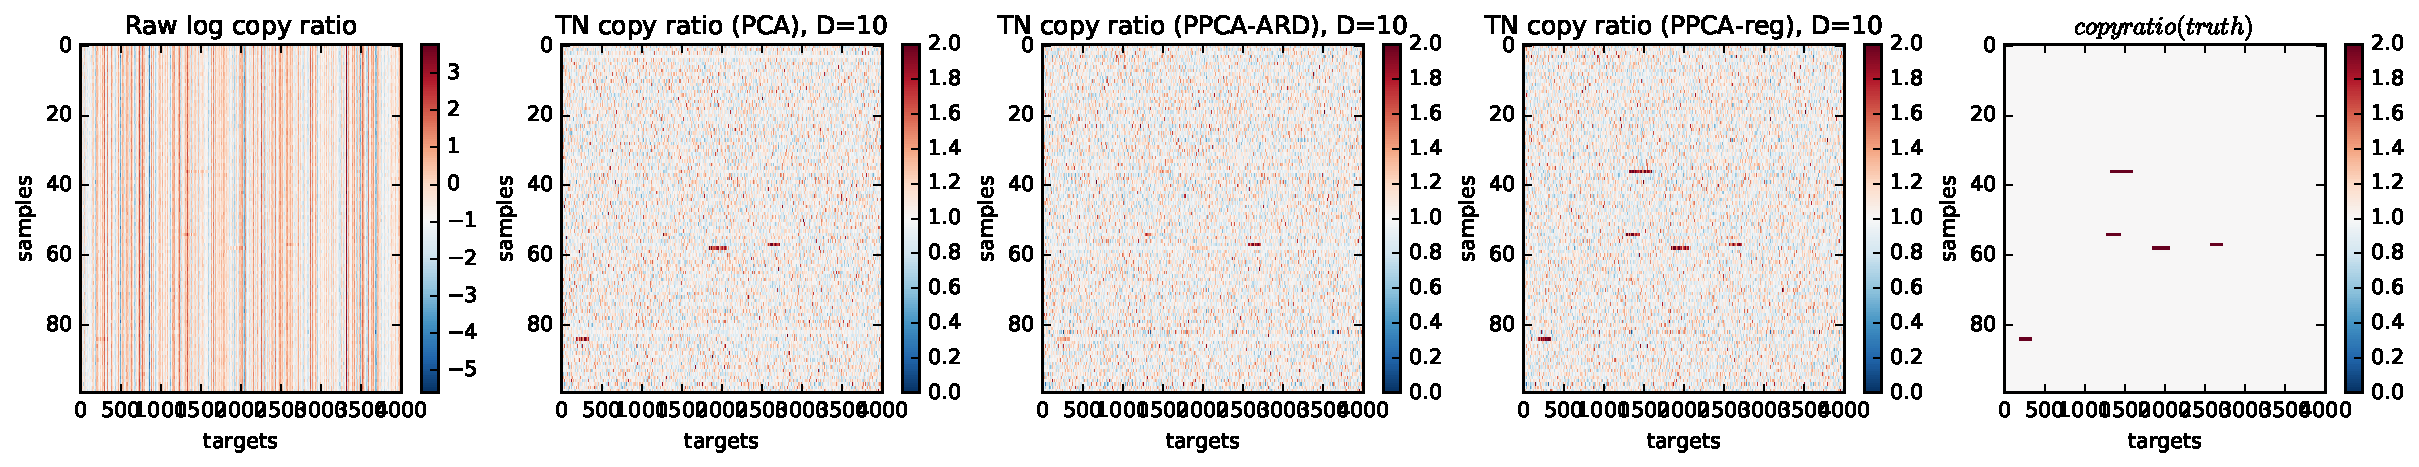
\includegraphics[scale=0.45]{figs/comp_random_events_10.pdf}
\vspace{20pt}
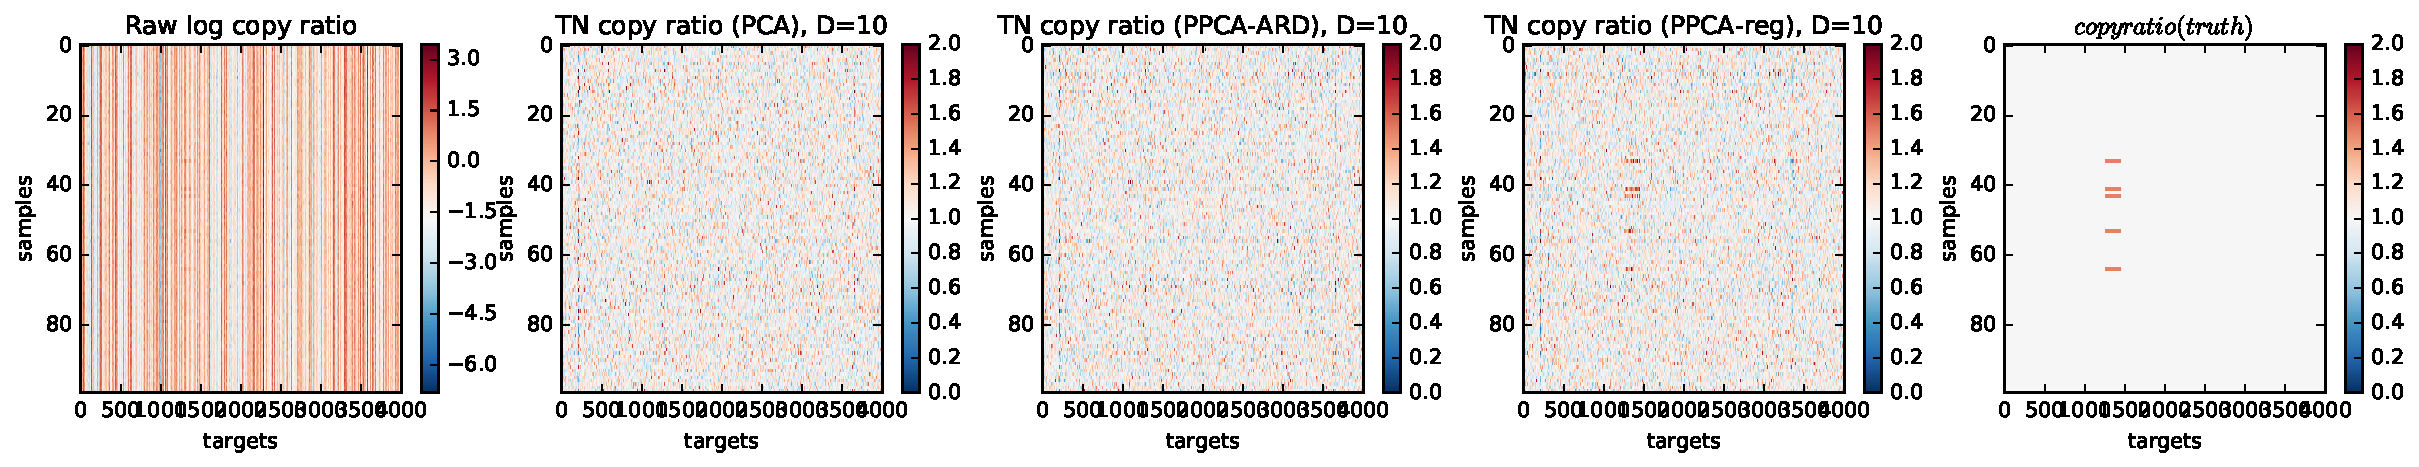
\includegraphics[scale=0.45]{figs/comp_corr_events_10.pdf}
$D=20$\\
\vspace{10pt}
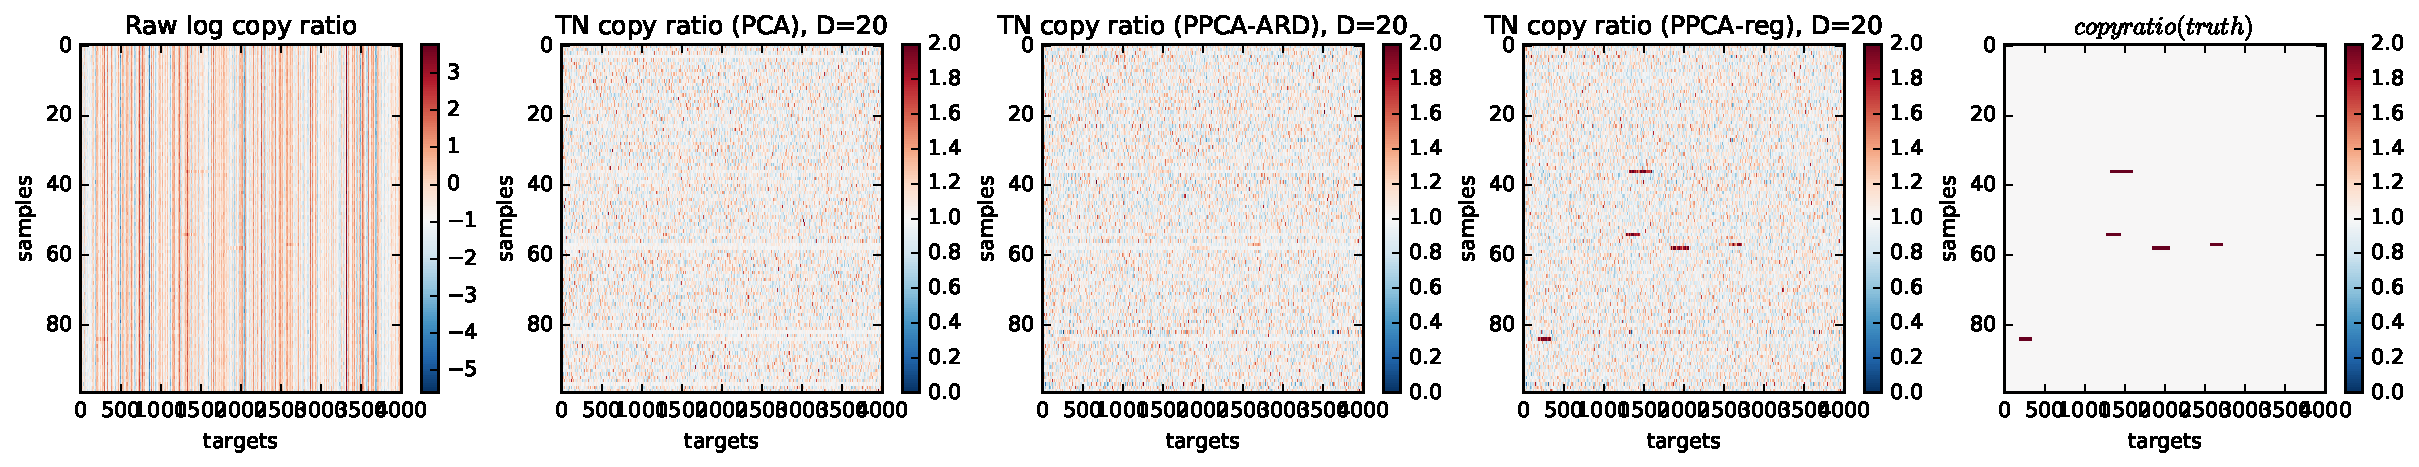
\includegraphics[scale=0.45]{figs/comp_random_events_20.pdf}
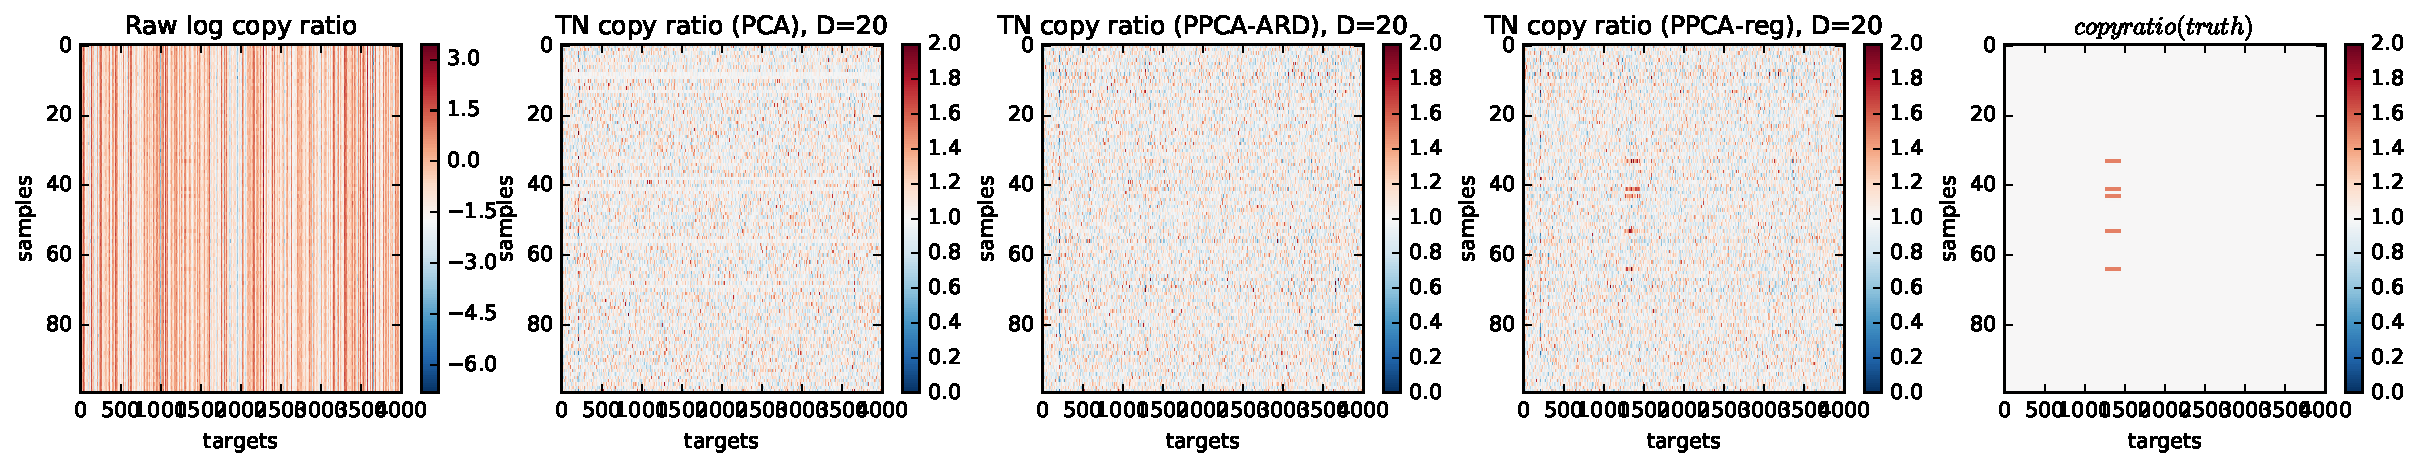
\includegraphics[scale=0.45]{figs/comp_corr_events_20.pdf}
\caption{Comparison of PCA with the probabilistic coverage model in different modes. Top two rows: $D=10$; random events, correlated events. Bottom two rows: $D=20$; random events, correlated events.}
\label{fig:comp_regularizer}
\end{figure}

\end{document}